


\documentclass[letterpaper]{article}
\usepackage{aaai}
\usepackage{times}
\usepackage{helvet}
\usepackage{courier}
\usepackage{xcolor}
\usepackage{cite }
\usepackage{graphicx, epsfig}
\usepackage[margin=1in]{geometry}
\usepackage[hyphens]{url}
\usepackage{enumitem}
\usepackage{amsmath}
\usepackage{algorithm}
\usepackage[noend]{algorithmic} % noend will ksip printing end of blocks

\usepackage{cite}
\usepackage{natbib}

\pagenumbering{gobble} %Do not print page numbers

\newcommand\ceg[1]{\textcolor{red}{#1}} % Red marker to declare errors.

\begin{document}

\title{Streaming Slot-Value Extraction for Wikipedia Entities at Web-Scale}

%\numberofauthors{3}




\author{Morteza Shahriari Nia, Christan Grant, Yang Peng, Daisy Zhe Wang\footnote{University of Florida, Gainesville, Florida, USA}, Milenko Petrovic\footnote{Institute for Human and Machine Cognition, Ocala, Florida, USA}\\
       \\
       {\{msnia, cgrant, ypeng, daisyw\}@cise.ufl.edu,}
       {mpetrovic@ihmc.us}
}

\maketitle


\begin{abstract}

% TODO this can be updated at the end

In this paper we will present the system design and algorithm adopted by the 
GatorDSR team, University of Florida to efficiently process TREC KBA 2013 --- 
SSF track. Here we will describe the system evolution as well as the details 
of our algorithm to extract slot values for the given slot name. Scalability 
and efficiency in precision and recall are the major   goals of this work, 
given the overly limited time limitation and available computational resources.

\end{abstract}



\section{Introduction}

Wikipedia.org (WP) is the largest and most popular general reference work on the Internet.
The website is estimated to have nearly 365 million readers worldwide.
An important part of keeping WP usable it to include new and current content.
%An important challenge in maintaining WP, the most popular web-based, collaborative, multilingual KB on the internet, is making sure its contents are up-to-date.
Presently, there is considerable time lag between the publication of an event and its citation in WP\@.
The median time lag for a sample of about 60K web pages cited by WP articles in the \textit{living\_people} category is over a year and the distribution has a long and heavy tail \cite{JFrank12}.
%Also, the majority of WP entities have updates on their associated article much less frequently than their mention frequency.
Such stale entries are the norm in any large reference work because the number
of humans maintaining the reference is far fewer than the number of entities.
Reducing latency keeps WP relevant and helpful to its users.
Given an entity page, such as \textit{wiki/Boris_Berezovsky_(businessman)}~\footnote{http://en.wikipedia.org/wiki/Boris_Berezovsky_(businessman)},
possible citations may come from a variety of sources.
Notable news may be derived from newspapers, tweets, blogs and a variety of different sources~\ref{}.
The actual citable information is a small percentage of the total documents that appear on the web.
%We develop a system to read streaming data and filter out articles that are candidates for citations. 
The goal of this system is to read web documents and recommend citable facts for WP pages.


Discovering arbitrary web pages that contain information that is relevant and citable 
to the WP entities is a non trivial task.
Entities from three categories of \textit{person}, \textit{organization} and \textit{facility} are considered.
% Reorder this paragraph
The challenges that we address are: first finding documents that contain useful information about the entity (avoid spams, documents that do not have direct information about the entity even though they mention them, etc), the scale where \textit{stream processing} nature of the system makes it suitable to avoid batch processing natures of Hadoop and operate in the realm of streams such as twitter storm~\footnote{http://storm-project.net/} which similarly processes unblounded streams of twitter data or Spark Streaming~\footnote{http://spark.incubator.apache.org/}. Further, this is called streaming because data is being generated as time goes
on and for each extraction we should only consider current or past data. As other Natural Language Processing tasks, precision and recall of the extent we can extract slot values are very important metrics that we will discuss later on. Having to balance between infamous and obscure entities, dealing with slots that can be very broad (e.g.\ things that an entity is affiliated with) or very specific (such as cause of death of a \textit{person} entity).

As an example, take a sentence from the internet \texttt{\underline{Boris Berezovsky} made his fortune in Russia in the 1990s when the country went through privatisation of state property and `robber capitalism', and passed away March 2013.}
First we have to pay attentions that there are two \textit{Boris Berezovsky} entities in WP, one a businessman and the other a pianist. Any slot value extraction shall take this into account and try to come up with a viable distinguishing policy (Entity Resolution). Then, we match the sentence to find a slot value such as \textit{DateOfDeath} valued at March 2013. Other examples that this system can answer could be `Who a person has met during a certain period of time?', `Who are the employees of this organization?', `Who has met who in this facility at a certain time?'.


In this paper we develop an efficient query-driven slot value extraction for given Wikipedia.org (WP) entities from a timely stream of documents on internet as they are being created. Slot value extraction is formally defined as follows: match each sentence to the generic sentence structure of [\textit{Subject} - \textit{Verb} - \textit{Adverbial/Complement}]\cite{sentencePatterns08}, where  \textit{Subject} represents the entity and \textit{Verb} is the relation type we are interested in (e.g. Table~\ref{table:slotNameOntology}). If a sentence matches these two components of the sentence pattern, \textit{Adverbial/Complement} would be returned as the other side of the relation (which we refer to as slot value). Slot value extraction is a challenging task in current state of the art Knowledge Bases (KB). Popular graphical KB such as Freebase or DBPedia keep data in structured format where entities are connected via relationships (\textit{Verb}) and the associated attributes (\textit{Adverbial/Compelement}). Our system can be used to automatically populate such KBs or even fill-in the information boxes at entity WP page itself.


Our system contains three main components. First, we pre-process the data and build models representing the WP query entities. Next, we use the models to filter a stream of documents so they only contain candidate citations. Lastly, we processes sentences from candidate extractions and return slot values. 
% EITHER SAY WHAT IT MEANS OR GIVE EXAMPLES OR COMMENT IT
%We build a modular system that allows us to explore the nuances of the training data and queries. 
Overall, we contribute the following:
\begin{itemize}[noitemsep,nolistsep]
\item Introduce a method to build models of name variations
\item Built a system to filter a large amount of diverse documents
\item Extract, infer and filter entity-slot-value triples of information to be added to KB 
\end{itemize}

\begin{table}
\caption{Ontology of Slots }
\centering
\label{table:slotNameOntology}

\setlength{\tabcolsep}{2pt}

\begin{tabular}{|c|c|c|}
\hline 
\textbf{Person} & \textbf{Facility} & \textbf{Organization} \\ 
\hline 
\begin{tabular}{@{}l@{}}Affiliate \\ AssociateOf \\  {\tiny Contact\_Meet\_PlaceTime} \\ AwardsWon \\ 
DateOfDeath \\ 
CauseOfDeath\\
Titles\\
FounderOf\\
EmployeeOf\end{tabular}
  &
   \begin{tabular}[b]{l}Affiliate \\ {\small Contact\_Meet\_Entity} \end{tabular} 
   & 
   \begin{tabular}{@{}l@{}}Affiliate \\ {\small TopMembers} \\ FoundedBy\end{tabular} \\ 
\hline 
\end{tabular} 
\end{table}
% Evaluation Criteria


% Quick Discussion of our approach




\section{System Overview}

In this section, we introduce the main components of the system. Our system is built with a pipeline architecture in mind giving it the advantage to run each section separately to allow stream processing without blocking the data flow of components (Figure~\ref{fig:system}). The three logical components include sections for performing preprocessing to prepare the required data, Cumulative Citation Recommendation to annotate cite-worthy documents, Streaming Slot Filling to generate the actual slot values and PostProcessing to increase precision/recall. We work on a streaming data set and entities are from Twitter or WP to query.


To walk you through the steps we take, assume we only care about on single WP entity, the first step is to extract aliases of the entity. We use several approaches to get as many viable aliases as possible. Then we look into the stream of content that is being generated on the internet, apply two levels of filtering to finally end up with the documents are central to that entity. To extract the relevnat slot values we perform pattern matching in each sentence or coreferent sentence to see if we can find a match. As a match is found from the content of the sentence to the patterns that we have generated regarding slot name, the associated slot value is extracted as a final result.

As mentioned before the time lag from an event occurance until it is cited in WP is in average over a year due to the fact that human maintainers are much less than the number of entities in WP and that the frequency of news update on entities escalates this difference. Hence having an automatic way to extract this knowldge for entities can be a very valuable asset.

%\ceg{Discuss current system first. If you want to keep the decisions points that led to the current architecture, make it a subsection.}

\begin{figure}
  \centering
%  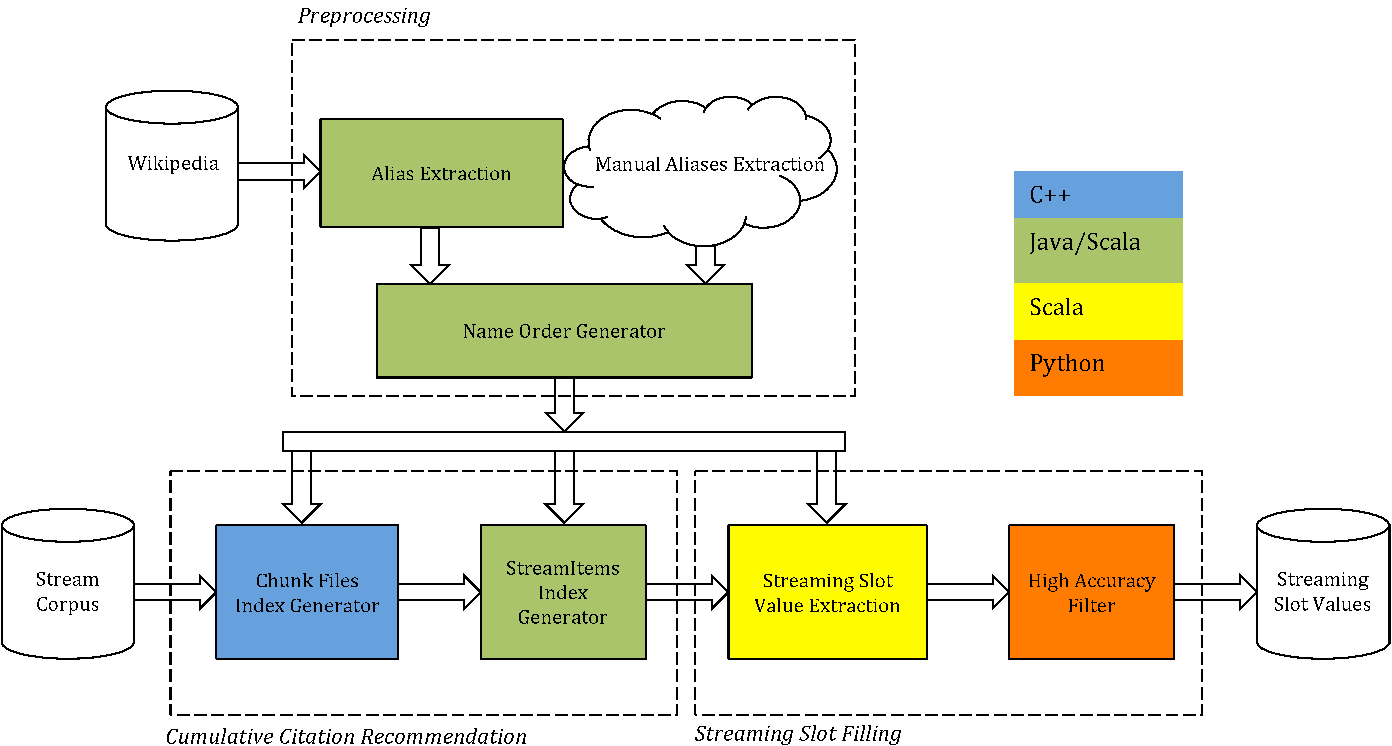
\includegraphics[width=6in]{./images/sdl-eps-converted-to.pdf}
  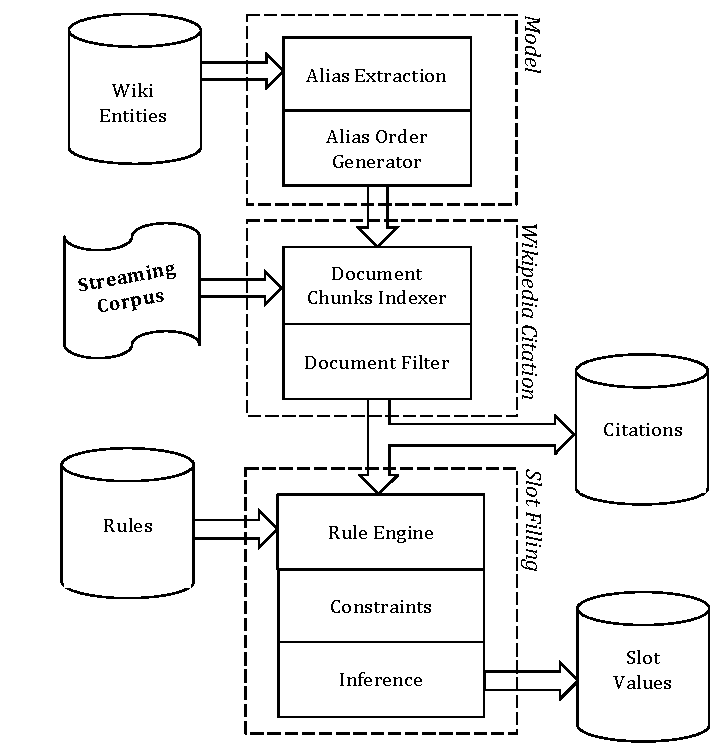
\includegraphics[width=3in]{./images/System_Diagram_with_model_Vertical-crop.pdf}
% http://convert.neevia.com/pdfconvert/
  \vspace*{-.1in} 
  \caption{The GatorDSR team System Architecture.
  Components are logically groups with dotted boxes.
  Color details the programing language implementation of components.}
  \label{fig:system}
  \vspace*{-.2in}
\end{figure}



\textit{Preprocessing.}
The contest prohibits Wikipedia entities to have any manual aliases being added and only allows automatic ways. We use Wikipedia API backlink references (redirects to a wiki entity) as aliases of the entity. We also extract aliases from within the text of a wiki entity, which will be described in Section~\ref{section:aliasgeneration}. This whole process is referred to as \textit{Alias Extraction}. The manual extraction rule is lifted and participants are allowed to manually add aliases for Twitter entities. This is allowed because the Twitter website does not provide an example page from the beginning of the document stream. This process of extracting aliases for Twitter entities is referred to as \textit{Manual Alias Extraction}.

Once aliases are available we pass them through rules of generating proper name orders which will produce various forms of writing a name. As a basic example Bill Gates can be written as Gates, Bill. This will allow the system to capture various notation forms of aliases. We refer to this part as \textit{Name Order Generator}.

\textit{Cumulative Citation Recommendation.}
The main goal of CCR is to have an aggregate list of documents that are worthy of being cited in a Wikipedia page. We perform exact string matching and treat all the documents that mention an entity equally likely to be citable. One of the reasons for this is that in former TREC KBA reports \cite{JFrank12} there were observations of how non-mentioning documents have a low chance of being citable in Wikipedia. So we take on that and ignore non-citing documents. 


% Note: Describe the algorithms of each phase
% Talk in abstract terms not implementation.
% Use formal representations (Math, SQL etc)


%\ceg{This section should be structured as follows:
%1: Introduce CCR (Motivation, Expectations)
%2: Our high level approach
%3: Discussion of our design (Like already discussed)
%}


\textit{Streaming Slot Filling.}
%\ceg{See the previous note.}
The purpose of SSF is to extract proper values for relations of interest, which can be found in Table~\ref{table:slotNameOntology}. This is called Stream Slot Filling because data is being generated as time goes
on and for each extraction we should only consider current or past data. In Figure~\ref{fig:system} we refer to this as \textit{Streaming Slot Value Extraction}. Stream slot filling is done by pattern matching documents with manually produced patterns for slots of interest. The way we do this is by observing a sentence that has a mention of the entity or one of its coreferences. An anchor word in the sentence related to the slot name is located and we match either left or right of the anchor word for potential slot values. 

\textit{Post Processing Algorithm.}
The SSF output of many extractions is noisy. The data contains duplicates and incorrect extractions. We can define rules to sanitize the output only using the information present in the SSF file. The file is processed in time order, in a tuple-at-a-time fashion to minimize the impact on accuracy. We define two classes of rules deduplication rules and inference rules. In our diagram we refer to this component as \textbf{High Accuracy Filter}.


%

\section{Implementation}
\label{section:implementation}

We extract aliases for entities from Wikipedia automatically both using API 
and using the actual page content, then apply pattern matching rules for slot 
value extraction. Our contribution is that we perform pattern matching that conforms to each slot 
value along with post-processings to eliminate noisy outputs. 

%\ceg{Instead of this paragraph we talk about what this %section will
%contain. We can discuss the input/output of the system %too.
%}

\subsection{Alias Generation}
\label{section:aliasgeneration}

We use Wikipedia API to get some aliases automatically. This is done by 
retrieving backlink references (redirects of a wiki entity). Unfortunately 
this is not good enough and to enhance recall we need more aliases. To have 
better use of a wiki page we parse HTML DOM of the page, then use regular 
expressions to extract the bold phrases of the first paragraph as alias of the 
actual entity. Based on our observation this is a very accurate heuristic and 
provides us with lots of famous aliases of the entities. To consider other 
typical cases we consider some generic first name last name order swapping 
conventions such as Bill Gates $\rightarrow$ Gates, Bill.  Meanwhile, William Henry Gates is an alias for Bill Gates in WP as a backlink reference. These kinds of aliases are also included in matching entities. 

\subsection{Streaming Slot Value Extraction}

\begin{figure}
\centering
%
\includegraphics[width=4.5in]{./images/system.eps}
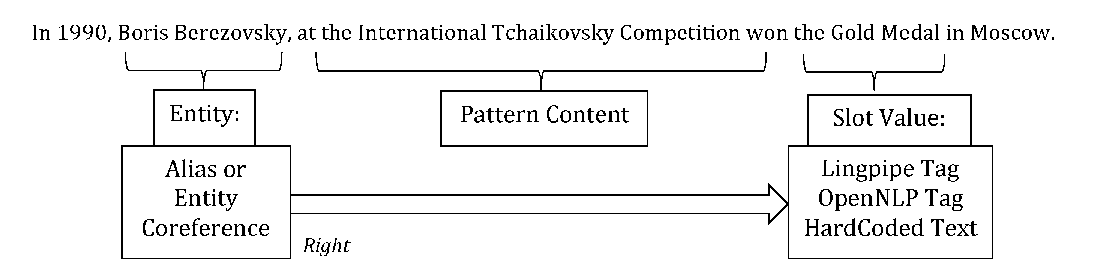
\includegraphics[width=6in]{./images/Pattern.eps}
\vspace*{-.1in} \caption{Pattern Matching with Slot Value on the Right Side of Entity. }\label{fig:pattern}
\vspace*{-.2in}
\end{figure}

In this system, we use pattern matching methods to find corresponding slot 
values for entities. This is done by observing the training data which is the first four months of the corpus (October 2011 - February 2012). The procedure is: First Find stream items that contain the 
entities by using alias names of the entities. Then Inside these stream items, 
fetch the sentences which contain entities by using alias names and the 
coreference information provided by Lingpipe tags. Use these sentences to 
match existing patterns, and when patterns matched, generate SSF results.

Each pattern consists of five fields:

\begin{itemize}
\item Type of the entity
\item Slot name
\item Pattern content
\item Direction of the slot value to the entity
\item Type of the slot values
\end{itemize}

 When we match one pattern, we match all the 
fields except the third field, which is extracted as the final result.

 The type of slot values could be the entity 
type tagged by Lingpipe, noun phrase tagged by OpenNLP and the time phrases we 
hard-code. For these three kinds of patterns, we implement them in different 
ways accordingly. Next we will explain the patterns with more details, a brief example can be found in Figure \ref{fig:pattern}. 

\textbf{Slot value type, tagged by Lingpipe:} For slot FounderOf, we have this
pattern: \textless \texttt{PER, FounderOf, founder, right, ORG}\textgreater. PER means 
that the entity we are finding slot values for is a PER entity; FounderOf 
means this is a pattern for FounderOf slot. Founder is the anchor word we are 
trying to match in the sentence text; right means that we are going to the 
right part of the sentence to match the pattern and find the slot value; ORG 
means the slot value should be a ORG entity.

\textbf{Slot value tagged as noun phrase by OpenNLP:} \textless \texttt{PER, AwardsWon, awarded, 
right, NP}\textgreater, NP meaning noun phrase. This pattern can be interpreted 
as that we are looking for a noun phrase after the “awarded'' since that noun 
phrase could possibly represent an award. Since titles and awards are usually 
not the Lingpipe entities, we use the OpenNLP noun phrase chunker to fetch the 
noun phrases.

\textbf{Slot value of time phrases, hard coded:} \textless \texttt{PER, DateOfDeath, died, right, 
last night}\textgreater. In this pattern, “last night'' means we are looking for 
exactly the phrase ``last night'' to the right of ``died''. This pattern is 
inspired by the intuition that in news articles, people often mention that 
somebody died last night instead of mentioning the accurate date information 
and Lingpipe tends not to tag phrases like ``last night'' as a DATE entity. 

To improve recall, we introduce generic patterns that can generate many results.
But these patterns generate many errors, too. Thus there is a trade-off 
between the accuracy and recall. This is one drawback of using pattern 
matching method, meaning it is really hard to find good patterns with both 
high accuracy and recall. 

For accuracy, we have found that there are three major kinds of errors: First,  
wrong entities found; next, wrong tags by the Lingpipe; and finally wrong results matched 
by the patterns. We solve the first problem by using the Wikipedia or twitter 
information of the entities to get better alias names. And we use
post-processing to reduce the second and third types of errors (Section \ref{section:highAccuracyFilter}).

\subsection{High Accuracy Filter}
\label{section:highAccuracyFilter}

The SSF output of many extractions is noisy. The data contains duplicates and 
incorrect extractions. We can define rules to sanitize the output only using 
the information present in the SSF file. The file is processed in time order, 
in a tuple-at-a-time fashion to minimize the impact on accuracy. We define 
two classes of rules: deduplication rules and inference rules.

The output contains many duplicate entries. As we read the list of extracted 
slots we create rules to define ``duplicate''. Duplicates can be present in a 
window of rows; we use a window size of 2 meaning we only be adjacent rows. 
Two rows are duplicates if they have the same exact extraction, or if the 
rows have the same slot name and a similar slot value or if the extracted 
sentence for a particular slot types come from the same sentence.

 New slots can be deduced from existing slots by defining inference rules. 
 For example, two slots for the task are ``FounderOf'' and ``FoundedBy''. A safe 
 assumption is these slot names are biconditional logical connectives with the 
 entities and slot values. Therefore, we can express a rule ``X FounderOf Y'' 
 equals ``Y FoundedBy X'' where X and Y are single unique entities. Additionally,
 we found that the slot names ``Contact\_Meet\_PlaceTime'' could be inferred as
 ``Contact\_Meet\_Entity'' if the Entity was a FAC and the extracted sentence 
 contained an additional ORG/FAC tag.  
We also remove erronious slots that have extractions that are several pages in 
length or tool small. Errors of extracting long sentences can typically be 
attributed to poor sentence parsing of web documents. We have some valid
``small'' extractions. For example a comma may separate a name and a title
(e.g. ``John, Professor at MIT''). But such extraction rules can be particularly 
noisy, so we check to see if the extracted values have good entity values.


% Note: Talk about how each of the algorithms were created

% Note: Give enough information for our algorithms to be
% reimplemented and verified.




\section{Evaluation}
\label{sec:results}

We evaluate the effectiveness of extracting slot values for 139 entities.
We look at the baseline coverage for entities and slot names we present in a 500M page snapshot of the English web.
We estimate the precision and recall of our extractions over several extracted fact. 

Our system was developed on a 32-core server described in Table~\ref{table:serverspec}.
Each document is annotated using a name entity extraction and in document coreference.
A bundle of documents are serialized into chunks and encrypted.
The total size of the data after compression and encryption is 4.5TB~\footnote{TREC Knowledge base acceleration stream corpus is available  \url{http://aws-publicdatasets.s3.amazonaws.com/trec/kba/index.html}}.
Data is ordered into 11952 date-hour buckets ranged from 2011-10-05-00 (5th of October 2011, 12am)
until 2013-02-13-23 (13th of Feburary 2013, 11pm).
The first four months of data (October 2011 - February 2012) is for training purposes, 
and we use this portion for rule and pattern creation and tuning.
The data set contains text from several web page types as listed in Table~\ref{table:documentsDist}.
%To have a sense of the scale of objects and compression as an example a 6mb gpg.xz files would become 45 mb thrift objects which can contain a couple of thousand StreamItems depending on their size.
%Some of the documents have null values for their annotation fields. The source code of our system is stored as an open source project where enthusiasts can also contribute to \cite{github}, also the relevant discussion mailing list is accessible here \cite{googlegroups}.
 
\begin{table}
\caption{Benchmark Server Specifications}
\centering
\label{table:serverspec}
\begin{tabular}{| c | p{4.8cm} |}
\hline 
\textbf{Spec} & \textbf{Details} \\ \hline
Model & Dell xxx 32 cores \\ \hline 
OS & CentOS release 6.4 Final \\ \hline 
Software Stack & GCC version 4.4.7, Java 1.7.0\_25, Scala 2.9.2, SBT 0.12.3 \\ \hline 
 RAM & 64GB\\ \hline 
 Drives & 2x2.7TB disks, 6Gbps, 7200RPM\\ \hline 
\end{tabular} 
\end{table}
 
\begin{table}
\caption{Document Chunks Distribution }
\centering
\label{table:documentsDist}

\begin{tabular}{|l|l|c|}
\hline 
\textbf{Document Type} & \textbf{\# of Documents} &  \textbf{Slots Found}\\ 
\hline 
Arxiv & 10988 & \\ \hline
 Classified & 34887 & \\ \hline
 Forum & 77674 & \\ \hline
 Linking & 12947 & \\ \hline
 Mainstream News & 141936 & \\ \hline
 Memetracker & 4137 & \\ \hline
 News & 280629 & \\ \hline
 Review & 6347 & \\ \hline
 Social & 688848 & \\ \hline
 Weblog & 740987 & \\ \hline
\hline 
\end{tabular} 
\end{table}


 
 
 
We develop 172 extraction patterns covering each slot-name/entity-type combinations.
%Our final submission was named \textit{submission\_infer}. 
%Our results are as follows: Document extraction using query entity matching with aliases, sentence extraction using alias matching and co-reference.
%Slot extraction using patterns, NER tags and NP tags.
Out of the 500 M documents and 139 entities we found 158,052 documents containing query entities, 17,885 unique extracted slot values for 8 different slots.
We did not get any results from 31 entities missing and 4 slots.

%On the performance of our initial submission run we performed random sampling via two processes, the results of which are according to Table~\ref{table:initialresult}.
In Table~\ref{table:initialresult} we performed two samples of a baseline submission and estimate the correctness of the extraction.
%\ceg{Add here how the baseline is different from the final submission}
We produced accuracies in range of  54\% and 55\%.
The errors present can be classified into two sets, incorrect entities and incorrect extractions.
We found 15\% and 17\% incorrect entity names and we identified 27\% and 30\% incorrect values extracted across all entities and slot types.
The majority of these errors were the result of poor extraction patterns and an incomplete alias set.

\begin{table}
\caption{Sampled accuracy of the results of the extracted facts.}
\centering
\label{table:initialresult}

\begin{tabular}{| c | c | p{2cm} | p{13mm} |}
\hline 
 & \textbf{Correct} & \textbf{Incorrect Entity name} & \textbf{Incorrect Value} \\ 
\hline 
Sampling \#1 & 55\% & 17\% & 27\% \\ 
\hline Sampling \#2 & 54\% & 15\% & 31\%  \\ 
\hline 
\end{tabular} 
\end{table}


%\ceg{Probably should add again here a reason why our method is different from the baseline.}
After the implementation of the baseline system, we developed an enhanced version. 
In this version we increased the number of extraction patterns and a generate a larger set of aliases.
More detailed statistics are available in Table~\ref{table:finalresultrecall} and Table~\ref{table:finalresultaccuracy}.
Table~\ref{table:finalresultrecall} shows the recall of each slot name. 
Entities can have different coverages across the entire web, some are more popular such as William H. Gates or less well known such as Stevens Cooperative School.
Similarly slot names have various coverages --- \textit{Affiliate} is more frequent compared to \textit{AwardsWon}. 
More sentences describing affiliate relationships exist across the WP entities than
sentences describing awards won. %\ceg{(define `entity coverage' here)}
The slot name \textit{Affiliate} has was extracted the most number of times and \textit{CauseOfDeath} was extracted the
fewest with 0 instances found matching the pattern list. \textit{AwardsWon} contained the next fewest with 38 instances found. 
Affiliate slot has a broad definition; any relation that directly connects an entity to another entity of any type can describe an Affiliate relationship.

%\begin{itemize}
%\item  any relation that is not of parent-child form, e.g. a sub-organization of an organization is not an affiliate of that organization but rather a member of.
%\item  A relationship consisting solely of the two groups
%interacting in a specific event context is not enough evidence to constitute a religious/political affiliation. 
%\item Former political or religious affiliations are correct responses for this slot. 
%\end{itemize}

To extract relationships such as affiliate is difficult because almost any
two items can be affiliated in some way.
%\ceg{Define the affiliate slot name.}
Our patterns for this relationship led to noisy results.
On the other hand for more precise slot names our accuracy increases but we have less recall.
Table~\ref{table:finalresultaccuracy} addresses the relative accuracy measure per slot value.
\textit{AssociateOf} has the highest accuracy with 63.6\% and  \textit{Affiliate}, \textit{Contact\_Meet\_PlaceTime} and \textit{EmployeeOf} have the lowest with lowest of 1\%, 1\% and 5\% accuracy respectively.
A discussion of different slots is available in literature \cite{tackbp}.


\begin{table}
\caption{Recall Measure: Generic slot names like affiliate had the most recall, compared to less popular slot names e.g. DateOfDeath}
\centering
\label{table:finalresultrecall}
\begin{tabular}{|l|p{13mm}|p{22mm}|}
\hline 
 \textbf{Slot Name} & \textbf{Instances Found} & \textbf{Entity \hspace{5 mm} Coverage} \\ 
\hline 
Affiliate & 108598 & 80 \\ \hline 
AssociateOf & 25278 & 106 \\ \hline 
AwardsWon & 38 & 14 \\ \hline 
CauseOfDeath & 0 & 0 \\ \hline 
Contact\_Meet\_Entity & 191 & 8 \\ \hline 
Contact\_Meet\_PlaceTime & 5974 & 109 \\ \hline 
DateOfDeath & 87 & 14 \\ \hline 
EmployeeOf & 75 & 16 \\ \hline 
FoundedBy & 326 & 30 \\ \hline 
FounderOf & 302 &  29 \\ \hline 
Titles & 26823 & 118 \\ \hline 
TopMembers & 314 & 26 \\ \hline 

\end{tabular} 



\caption{Accuracy Measure: Accuracy of AffiliateOf was the best and Affiliate applied poorly due to ambiguity of being an affiliate of somebody/something}
\centering
\label{table:finalresultaccuracy}
\begin{tabular}{|l|p{10mm}|p{10mm}|p{11mm}|}
\hline 
 \textbf{Slot Name}  & \textbf{Correct} & \textbf{Wrong Entity} & {\small \textbf{Incorrect Value}} \\ 
\hline 
Affiliate & 1\% & 95\% & 5\% \\ \hline 
AssociateOf & 63.6\% & 9.1\% & 27.3\%  \\ \hline 
AwardsWon & 10\% & 10\% & 80\%  \\ \hline 
CauseOfDeath & 0\% & 0\% & 0\%  \\ \hline 
Contact\_Meet\_Entity & 21\% & 42\% & 37\%  \\ \hline 
Contact\_Meet\_PlaceTime & 5\% & 20\% & 85\%  \\ \hline 
DateOfDeath & 29.6\% & 71\% & 25\%  \\ \hline 
EmployeeOf & 5\% & 30\% & 65\%  \\ \hline 
FoundedBy & 62\% & 17\% & 21\%  \\ \hline 
FounderOf & 50\% & 0\% & 50\%  \\ \hline 
Titles & 55\% & 0\% & 45\%  \\ \hline 
TopMembers & 33\% & 17\% & 50\%  \\ \hline 

\end{tabular} 
\end{table}








% Note: Here is where we give as much stats as possible on our runs





\section{Discussion}

As mentioned before, when we evaluate the results of slot extraction, we find three kinds of problems for accuracy: 1) wrong entities found; 2) wrong tags by the Lingpipe; 3) wrong results matched by the patterns.  We also have recall problems: 1) not enough good alias names to find all the entities. 2) not enough and powerful patterns to capture all the slot values. 

We will use entity resolution methods and other advanced methods to improve the accuracy and recall of entity extraction part. 

For slot extraction part, in order to improve the performance, what we need to are: 1) Using multi-class classifiers instead of pattern matching method to extract slot values in order to increase both recall and accuracy for slots “Affiliate”, “AssociateOf”, “FounderOf”, “EmployeeOf”, “FoundedBy” “TopMembers”, “Contact\_Meet\_Entity” and so on. 2) For special slots, like “Titles”, “DateOfDeath”, “CauseOfDeath”, “AwardsWon”, using different kind of advanced methods, e.g. classifiers, matching methods. 3) Using other NLP tools or using classifiers to overcome the drawbacks of the LingPipe’s inaccurate tags. The first and second tasks are the most important tasks we need to do.

% Note: Here we discuss why the results are the way they are
% Give pros and cons, talk about how the implemented algorithms
% performed in the actual implementation.
% Answer the `why' question about all the trends in the results section.




\section{Conclusion}

In this paper we described an approach to perform fact extraction over one of the largest data sets to date. 
We generate aliases for Wikipedia entities using an API and extract some aliases from Wikipedia pages text itself.
We process documents that mention entities for slot value extraction.
Slot values are determined using pattern matching over tagged entities in sentences.
Finally post processing will filter, cleanup and infers some new slot values to enhance recall and accuracy. 

We sampled documents from the training data period to generate an initial set of patterns and then use these patterns to generate results.
After manually examining the results, we prune patterns with poor performance and add patterns that may add to extraction coverage.
We use several iterations to find the best patterns.
%We found that it is very time consuming to identify quality patterns.

%We noticed that some tools that claim to be performant for using the hardware capabilities at hand sometimes don't really work as claimed and you should not always rely on one without a thorough A/B testing of performance which we ended up in generating our in-house system for processing the corpus and passing through the filter. Furthermore, on extracting slot values, pattern matching might not be the best options but definitely can produce some good results at hand. We have plans on generating classifiers for slot value extraction purposes. Entity resolution on the other hand was a topic we spent sometime on but could not get to stable grounds for it. Entity resolution will distinguish between entities of the same name but different contexts. Further improvements on this component of the system are required. 


We look to continue exploration of streaming extraction models over this large data set.
Our models are simple and provide a great baseline framework to develop and compare innovative techniques.



% Note: Give a summary of our efforts and the
% high level contribution to society.

% Talk about the things we wanted to do and
% didnt get to do.



\section*{Acknowledgements}
Christan Grant is funded by a National Science Foundation Graduate Research Fellowship under Grant No. DGE-0802270. 

%\bibliographystyle{acm}
%\bibliography{citation}

\bibliography{citation}
\bibliographystyle{aaai}

%

\appendix

\section{KBA Task Background}
\label{sec:kbatask}
The National Institute of Standards (NIST) hosted the
Text REtrieval Conference (TREC) --- Knowledge Base Acceleration challenge in 2013. The task
contains two main sections designed for this track, Cumulative Citation Recommendation 
and Streaming Slot Filling. Due to the importance of knowledge bases, both of these 
tracks aim to accelerating populating them, hence the title Knowledge Base Acceleration (KBA).
Below we describe each of these tracks and their purposes.

\subsection{Cumulative Citation Recommendation (CCR)}

For this track, assessors were instructed to ``use the Wikipedia article to 
identify (disambiguate) the entity, and then imagine forgetting all info in the WP 
article and asking whether the text provides any information about the entity'' \cite{JFrank12}.
Documents are divided according if an entity is mentioned and a relevance level to the entity.

More specifically, a document may have a mention or be without a mention.
\begin{itemize}[noitemsep]
  \item \textbf{Mention:} Document explicitly mentions target entity, such as full 
    name, partial name, nickname, pseudonym, title, stage name.
  \item \textbf{Zero-mention:} Document does not directly mention target. Could 
    still be relevant, e.g.\ metonymic references like ``this administration'' 
    $\rightarrow$ ``Obama''. See also synecdoche. A document could also be relevant to 
    target entity through relation to entities mentioned in document -- apply this 
    test question: can I learn something from this document about target entity using 
    whatever other information I have about entity?
\end{itemize}

The relevance of a document to a query is split into the four classifications.
\begin{itemize}[noitemsep]
  \item \textbf{Garbage:} not relevant, e.g.\ spam.
  \item \textbf{Neutral:} Not relevant, i.e.\ no info could be deduced about entity, 
    e.g., entity name used in product name, or only pertains to community of target 
    such that no information could be learned about entity, although you can see how 
    an automatic algorithm might have thought it was relevant.
  \item \textbf{Relevant:} Relates indirectly, e.g., tangential with substantive 
    implications, or topics or events of likely
    impact on entity.
  \item \textbf{Central:} Relates directly to target such that you would cite it in 
    the WP article for this entity, e.g.\ entity is a
    central figure in topics/events.
\end{itemize}


\subsection{Streaming Slot Filling (SSF)}
The task is that given certain WP or Twitter entities 
(wiki/twitter URLs) and certain relations of interest (given in
Table~\ref{table:slotNameOntology}), extract as many triple relations as possible (
hence, slot filling). This can be used to automatically populate knowledgebases 
such as free-base or DBPedia or even fill-in the information boxes at Wikipedia. 
Below, you can view some examples of what it means to fill in a slot value; in 
each example there is a sentence of interest that we wish to extract slot values 
from, an entity that the slot value is related to, and a slot name which can be 
thought of as the topic of the slot value:

\noindent \textbf{Example 1:} ``Matthew DeLorenzo and Josiah Vega, both 14 years old and students 
at Elysian Charter School, were honored Friday morning by C-SPAN and received 
\$1,500 as well as an iPod Touch after winning a nationwide video contest.''

Entity:  http://en.wikipedia.org/wiki/Elysian\_Charter\_School

Slot name: Affiliate

Possible slot values: ``Matthew DeLorenzo'', ``Josiah Vega''

Incorrect slot values: ``C-SPAN'', ``iPod Touch''

\noindent \textbf{Example 2:} ``Veteran songwriters and performers Ben Mason, Jeff Severson and 
Jeff Smith will perform on Saturday, April 14 at 7:30 pm at Creative Cauldron 
at ArtSpace, 410 S. Maple Avenue.''

Entity: http://en.wikipedia.org/wiki/Jeff\_Severson

Slot name: Affiliate

Possible slot values: ``Ben Mason'', ``Jeff Severson'', ``Jeff Smith''

Incorrect slot values: ``Creative Caldron'', ``Art Space''

\noindent \textbf{Example 3:}  ``Lt. Gov. Drew Wrigley and Robert Wefald, a retired North Dakota 
district judge and former state attorney general, unveiled the crest Friday 
during a ceremony at the North Dakota Capitol.''

Entity: http://en.wikipedia.org/wiki/Hjemkomst\_Center

Slot name: Contact\_Meet\_PlaceTime

Slot value: ``Friday during a ceremony at the North Dakota Capitol''


\noindent In \textit{streaming} slot filling, we are only interested in new 
slot values that were not substantiated earlier in the stream corpus.
In Table~\ref{table:slotNameOntology} you can view some slot values 
and their types, the comprehensive description of which can be found at
\cite{tackbp} and \cite{aec}. The details of the metric for SSF will favor systems 
that most closely match the changes in the ground truth time line of slot values. 
This is done by searching for other documents that mentioned an entity and exactly 
matched the slot fill strings selected by the assessors.



%In the rest of the paper, we address the following material. In Section 2, we 
%sketch the main components of the system and their purposes. In Section 3, 
%describe the details of how we designed and implemented certain components 
%critical to the behavior of the system. Section 4 addresses the performance and 
%the results we achieved. Section 5, goes through a discussion of the challenges we 
%had to produce reliable results over the massive amount of information available, 
%and how we overcome these issues.
For similar approaches regarding last year's track you can refer to \cite{ji2011knowledge}.

%\ceg{Add a discussion of why machine driven kb population is important.}


\begin{table}[h]
\caption{Ontology of Slot Name Categories }
\centering
\label{table:slotNameOntology}

\begin{tabular}{|c|c|c|}
\hline 
\textbf{PER} & \textbf{FAC} & \textbf{ORG} \\ 
\hline 
\begin{tabular}{@{}l@{}}Affiliate \\ AssociateOf \\ Contact\_Meet\_PlaceTime \\ AwardsWon \\ 
DateOfDeath \\ 
CauseOfDeath\\
Titles\\
FounderOf\\
EmployeeOf\end{tabular}
  &
   \begin{tabular}[b]{l}Affiliate \\ Contact\_Meet\_Entity \end{tabular} 
   & 
   \begin{tabular}{@{}l@{}}Affiliate \\ TopMembers \\ FoundedBy\end{tabular} \\ 
\hline 
\end{tabular} 
\end{table}


%\ceg{How will each submission be evaluated?}

% Motivation


% KBA Task






\end{document}
